\paragraph{}
En este apartado se desarrollar\'an los diferentes módulos que componen el sistema.
Como se ha introducido en el apartado \ref{sec:intro}, el sistema de comunicaciones consta de un emisor y receptor que comparten la misma estructura de diseño: 
una parte analógica que actúa como la interfaz de comunicación de radiofrecuencia y una parte digital que trabaja con las señales banda base. Además, la parte digital también se encarga de la codificación y decodificación del enlace.
\paragraph{}
En cuanto a la parte analógica de radiofrecuencia nos encontramos las siguientes características generales que se desarrollan en los consiguientes apartados. 
La comunicaci\'on que se llevará a cabo consiste en un enlace digital mediante radio frecuencia de dos canales.
La frecuencia de trabajo es de \SI{30}{\mega\hertz} sobre una modulación es ASK.
Esta modulación implica que el sistema analógico de radio trabaja recibiendo tonos sintonizados a la frecuencia de trabajo.
\paragraph{}
Por otro lado, la parte digital, trabaja tanto con
la codificación en la parte emisora, como con demodulación de las señales digitales en la parte receptora. 
La codificación y demodulación se realiza con ayuda de un microcontrolador Atmega328p, el cual, mediante las señales producidas por dos distintos pulsadores, codifica la señal digital de manera NRZ apolar.
Esta señal es posteriormente demodulada y decodificada en el receptor.
\paragraph{}
En la figura \ref{fig:bloques_gral}, se muestra un diagrama de bloques como esquema general de ambas partes del proyecto, transmisor y receptor. En ambos casos se diferencian la parte digital y anal\'ogica en cada caso.

\begin{figure}[h]
    \centering
    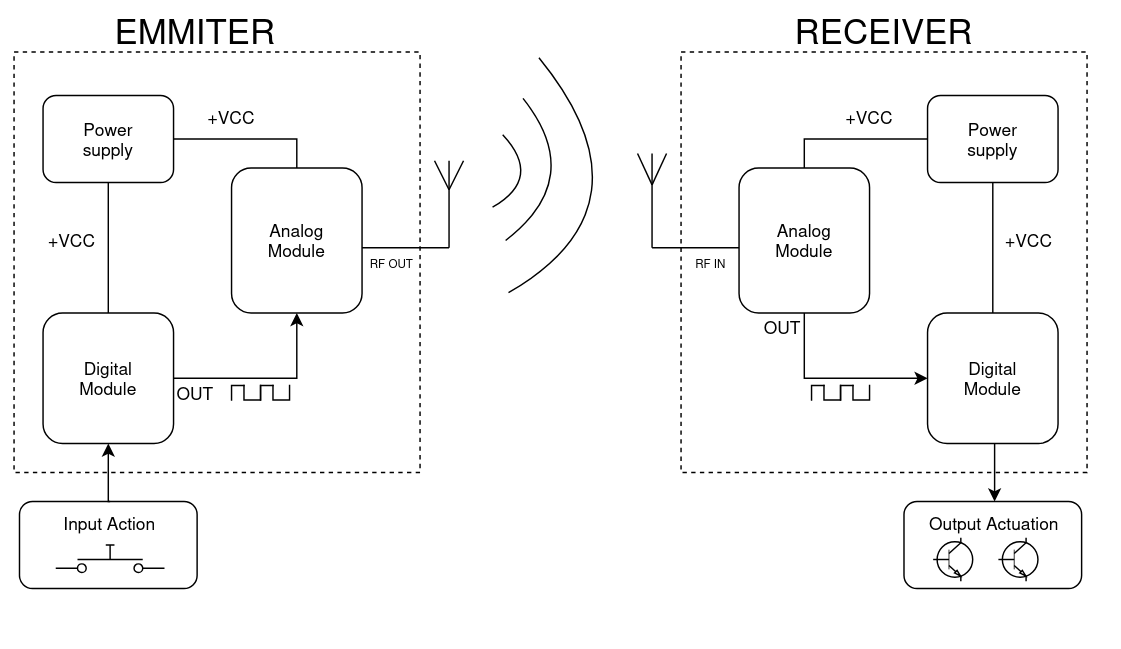
\includegraphics[scale=1, width=1\textwidth]{bloques_gral}
    \caption{Diagrama de bloques general del proyecto}
    \label{fig:bloques_gral}
\end{figure}
